%% —---------------------------------------------------
%% sbcreviews-en.tex
%% Template for SBC Reviews 
%% (https://journals-sol.sbc.org.br/index.php/reviews/) 
%% 
%% A versão do template inclui algumas
%% modificações sobre o template original da REIC
%% (https://journals-sol.sbc.org.br/index.php/reic)
%%
%% Licença: CCBY 4.0 
%% (https://creativecommons.org/licenses/by/4.0/)
%% Sociedade Brasileira de Computação.

\documentclass[english]{sbcreviews-2025}%

\usepackage[misc,geometry]{ifsym} 

%\usepackage{graphicx} % carregada dentro da classe
%\usepackage{fontspec} % carregada dentro da classe
%\usepackage{fontawesome} % carregada dentro da classe
%\usepackage{color} % carregada dentro da classe
%\usepackage{hyperref} % carregada dentro da classe

\usepackage{aas_macros}
\usepackage[bottom]{footmisc}

\usepackage{tabularray}
% O pacote tabularray torna o uso dos pacotes abaixo desnecessarios.
%\usepackage{supertabular}
%\usepackage{multicol}
%\usepackage{multirow}

\usepackage{afterpage}
\usepackage{url}
\usepackage{pifont}

\usepackage{array,booktabs,tabularx,threeparttable}
\newcolumntype{Y}{>{\raggedright\arraybackslash}X}

% Códigos compactos para Specialization (use onde preferir)
\newcommand{\GP}{\textbf{GP}}   % General-purpose
\newcommand{\AG}{\textbf{AG}}   % App Generation
\newcommand{\FE}{\textbf{FE}}   % Frontend-only
\newcommand{\AU}{\textbf{AU}}   % Automation
\newcommand{\CA}{\textbf{CA}}   % Code Analysis
\newcommand{\SQ}{\textbf{SQ}}   % SQL-only
\newcommand{\WP}{\textbf{WP}}   % WordPress
\newcommand{\PY}{\textbf{PY}}   % Python
\newcommand{\AN}{\textbf{AN}}   % Android
\newcommand{\CJ}{\textbf{CJ}}   % COBOL \& Java
\newcommand{\RE}{\textbf{RE}}   % Regex
\newcommand{\WG}{\textbf{WG}}   % Website Generation
\newcommand{\PJ}{\textbf{PJ}}   % Python \& JS/TS

% Macro opcional para facilitar os triplos (ID, Nome, Cod)
\newcommand{\Tech}[3]{#1 & #2 & #3}

\setcitestyle{square}

\definecolor{engtitle}{rgb}{0.5,0.5,0.5}
\definecolor{orcidlogo}{rgb}{0.37,0.48,0.13}
\definecolor{unilogo}{rgb}{0.16, 0.26, 0.58}
\definecolor{maillogo}{rgb}{0.58, 0.16, 0.26}
\definecolor{darkblue}{rgb}{0.0,0.0,0.0}
\hypersetup{colorlinks,breaklinks,
            linkcolor=darkblue,urlcolor=darkblue,
            anchorcolor=darkblue,citecolor=darkblue}
%\hypersetup{colorlinks,citecolor=blue,linkcolor=blue,urlcolor=blue}
% We disable hyperlinks by default with this line, to avoid the error "\pdfendlink ended up in different nesting level" while writing

\jid{ROCS}
\jtitle{SBC Computing Reviews, 2025, XX:1}
\issn{2966-3938}
\doi{10.5753/rocs.202X.XXXXXX}
\copyrightstatement{This work is licensed under a Creative Commons Attribution 4.0 International License}
\jyear{202X}

\category{Review}

\title[AI Solutions Applicable to Software Construction - A Rapid Multivocal Review]{AI Solutions Applicable to Software Construction - A Rapid Multivocal Review}

%THE ORCID IS MANDATORY FOR EACH AUTHOR IN ROCS
\author[Assis et al. 2025]{
\affil{\textbf{Felipe Assis}~\orcidlink{0009-0001-0113-6239}~\textcolor{blue}{\faEnvelope}~~[{Universidade Federal do Rio de Janeiro}~|\href{mailto: ...}{~{\textit{fassis@cos.ufrj.br}}}~]}

\affil{\textbf{Júlio César Guimarães}~\orcidlink{0009-0004-8626-5970}~[{Universidade Federal do Rio de Janeiro}~|\href{mailto: ...}{~{\textit{jcguimaraes@cos.ufrj.br}}}~]}

\affil{\textbf{Sabrina Rocha}~\orcidlink{0000-0002-4894-6095}~[{Universidade Federal do Rio de Janeiro}~|\href{mailto: ...}{~{\textit{sabrinarocha@cos.ufrj.br}}}~]}

\affil{\textbf{Rodrigo Feitosa Gonçalves}~\orcidlink{0000-0003-0960-3126}~[{Universidade Federal do Rio de Janeiro}~|\href{mailto: ...}{~{\textit{rfeitosa@cos.ufrj.br}}}~]}

\affil{\textbf{Guilherme Horta Travassos}~\orcidlink{0000-0002-4258-0424}~[{Universidade Federal do Rio de Janeiro}~|\href{mailto: ...}{~{\textit{ght@cos.ufrj.br}}}~]}

}

\begin{document}

\begin{frontmatter}

\maketitle

\begin{mail}
Avenida Horácio Macedo 2030, Centro de Tecnologia, Bloco H, sala 319 - Cidade Universitária - CEP: 21941-914 
\end{mail}


\begin{abstract-en}
This study conducts a Rapid Multivocal Review (RMR) to systematically map Generative AI solutions applicable to software construction, integrating both academic and grey
literature sources. The primary aim is to clarify the broader capabilities, practical accessibility, maturity levels, and limitations of AI-driven tools beyond conventional code generation. Utilizing a structured PICOC-based search strategy and advanced filtering
methods, the review identifies 156 relevant Generative AI tools and categorizes them by usage context, including general-purpose tools, frontend-only solutions, and more robust app-generation platforms. The findings highlight varying maturity levels, ranging
from widely adopted commercial tools to experimental prototypes. Key challenges identified include technical limitations related to context-awareness, operational constraints due to integration complexity and cloud dependencies, and legal concerns regarding data privacy. Future directions suggest extending the scope through additional repositories, integrating practitioner feedback, establishing automatic refinement loops, and enhancing classification methods with reinforcement learning. Continuous evaluation and updates are crucial, given the rapid technological evolution in Generative AI, to maintain relevance and practical
applicability.
\end{abstract-en}

\begin{keywords}
Generative Artificial Intelligence, Software Construction, Large Language Model, AI Tool
\end{keywords}


%\begin{dates}
% This information will be provided by the editor befeore publishing the paper
%\noindent{\sffamily\textbf{Received:}} DD Month YYYY~~~$\bullet$~~~
%${\sffamily\textbf{Accepted:}} DD Month YYYY~~~$\bullet$~~~
%{\sffamily\textbf{Published:}} DD Month YYYY
%\end{dates}


%\begin{license}
%Published under the Creative Commons Attribution 4.0 International Public License (CC BY 4.0)
%\end{license}

\end{frontmatter}


% =================================================================
% Introduction
% =================================================================
\section{Introduction}\label{sec:intro}
Generative Artificial Intelligence (AI), particularly through Large Language Models (LLMs), has recently emerged as a significant topic in both academic research and industry discussions, driven by its potential to enhance software development practices substantially. Traditionally, software construction involves manual coding, repetitive tasks, and significant clerical work. These activities can be notably improved through Generative AI-driven automation. Tools such as GitHub Copilot and Tabnine have demonstrated practical benefits in automating code generation, improving developer productivity, and reducing cognitive load, as supported by empirical studies examining developers' perceptions and the effectiveness of these tools \cite{sergeyuk2025using}.

However, while automated code generation has received considerable attention, software construction involves a broader set of tasks, including code structuring, refactoring, adapting to evolving requirements, and maintaining architectural coherence and consistency. Despite recognizing the potential benefits of Generative AI, there remains limited clarity regarding its broader capabilities, practical accessibility, maturity levels, limitations, and overall applicability to these software construction tasks beyond mere code generation.

This paper addresses this gap by conducting a Rapid Multivocal Review (RMR) \cite{rocha2025metaprotocol}, mapping the landscape of Generative AI tools and methods explicitly related to software construction. The review aims to provide valuable insights for both academic researchers and industry practitioners seeking to improve their software development processes.


% =================================================================
% Related Work
% =================================================================
\section{Related Work}\label{sec:relatedwork}
The field of research on code generation with artificial intelligence has been growing exponentially in recent years. Both academia and industry have produced numerous proposals, tools, and models to support this activity, making it one of the most dynamic topics in contemporary software engineering. This scenario highlights a rapidly evolving field that necessitates new research capable of providing timely, comprehensive reviews of available code-generation options and their specific details. Given the breadth of recent publications, for the sake of objectivity, this article highlights only a few works directly relevant to the topic, without attempting to exhaust the entire body of literature in the area.

\cite{jiang2024survey} presents a systematic and comprehensive review of the state of the art in language models applied to code generation. In addition to proposing a taxonomy that covers data curation, technical advances, and even ethical and environmental impacts, the study also provides a chronological overview of the evolution of large language models for code generation in recent years, highlighting the rapid succession of innovations in this field. This work relates to the present article by demonstrating the consolidation of code generation as its own research line, with accelerated expansion, serving as a foundation for identifying advances and gaps that still require further exploration, especially regarding empirical evaluation and the gap between academia and industrial practice.

\cite{liu2024large} broadens the discussion by analyzing the use of LLM-based agents in the context of software engineering. In addition to positioning agents as a new paradigm—where models are combined with mechanisms of planning, memory, perception, and action to deal with complex tasks—the study provides a comprehensive overview of their application in different software engineering tasks, including code generation, and lists several agents and tools that have been employed for this purpose. This perspective is relevant because it shows a trend in the evolution of LLM usage, from simple code-generation assistants to autonomous systems capable of acting across end-to-end development processes.

\cite{sergeyuk2025using} offer a more applied perspective and are closer to the idea of the present article, as they investigate how industry is using artificial intelligence for code generation. However, this analysis was conducted through interviews with 481 developers, which enabled the mapping of perceptions, practices, and limitations of these assistants in everyday software development. The authors highlight which activities programmers prefer to delegate to AI, as well as the reasons why these assistants are not used in certain stages, such as a lack of trust or contextual limitations. This work complements previous work by providing practical evidence of adoption and the challenges faced in real-world development environments, offering a user-centered, practice-oriented perspective.

Finally, unlike the highlighted works, this article does not aim solely to systematize technical advances or gather usage perceptions. Instead, it distinguishes itself by proposing a rapid and multivocal review. By adopting this approach, the goal is to capture not only what the formal academic literature has discussed but also perspectives from technical reports, specialized blogs, and other industry sources, aiming to provide a broader and more up-to-date view of what is effectively being used in terms of artificial intelligence for code generation, thus accelerating the understanding of the current state of this constantly evolving field.

% Multivocal literature reviews have increasingly gained attention as methods to integrate insights from both academic literature and grey literature, providing richer and broader perspectives on technological topics. In software engineering and related areas, several studies have successfully demonstrated the value of multivocal reviews for understanding complex phenomena involving AI technologies. For example, Felizardo and Carver \cite{felizardo2020automating} outline automated systematic literature reviews in software engineering, emphasizing the importance of considering diverse information sources to ensure comprehensive analyses.

% Cartaxo et al. \cite{cartaxo2020rapid} discuss how rapid reviews can efficiently summarize evidence to support timely decision-making in dynamic fields such as software engineering. Moreover, Garousi et al. \cite{garousi2020grey} explicitly address the significance of incorporating grey literature into software engineering research, arguing that industrial and practitioner-driven insights enrich the applicability and context-relevance of findings.

% In the broader AI context, similar methodological frameworks have been applied. Previous work \cite{swbokv4} has emphasized the evolving role of generative models and large language models, underscoring the relevance of multivocal approaches to stay updated with rapidly evolving AI capabilities. Thus, this rapid multivocal review not only draws from these methodological precedents but also expands upon them by specifically examining the state-of-the-art and practice of generative AI solutions applicable to software construction.


% =================================================================
% Research Method
% =================================================================
\section{Research Method}\label{sec:researchmethod}
Multivocal literature reviews have gained increasing attention as methods for integrating insights from both academic and grey literature, providing richer and broader perspectives on technological topics. In software engineering and related areas, several studies have successfully demonstrated the value of multivocal reviews for understanding complex phenomena involving AI technologies. For example, \cite{felizardo2020automating} outline automated systematic literature reviews in software engineering, emphasizing the importance of considering diverse information sources to ensure comprehensive analyses.

\cite{cartaxo2020rapid} discuss how rapid reviews can efficiently summarize evidence to support timely decision-making in dynamic fields such as software engineering. Moreover, \cite{garousi2020grey} explicitly address the significance of incorporating grey literature into software engineering research, arguing that industrial and practitioner-driven insights enrich the applicability and context-relevance of findings.

This research employs a Rapid Multivocal Review (RMR) methodology, inspired by contemporary guidelines for multivocal literature reviews in Software Engineering (SE) ~\cite{cartaxo2020rapid,felizardo2020automating,garousi2020grey}. Given the rapid evolution and widespread adoption of Generative Artificial Intelligence (AI) within software engineering, this methodology is tailored specifically to leverage automated filtering and address the considerable volume and diverse nature of sources, encompassing both academic and grey literature.

\subsection{Definition of Goal and Research Question}

The primary goal of this RMR is to systematically identify and map Generative AI-based solutions available to support software construction activities in both academic and industrial contexts. The central research question guiding this review is:


\begin{quote}
\textbf{RQ1}: \textit{Which Generative AI-based solutions (tools, agents, models, etc.) are available to support software engineering activities, particularly software construction, within industry and academia?}
\end{quote}

This central question is further detailed into eight sub-questions (RQ1a–RQ1h), addressing applicability, accessibility, usage models, limitations, and maturity:

\begin{itemize}
    \item \textbf{RQ1a:} \textit{Where can these solutions be found?}  
    \textbf{Rationale}: Identifying the distribution channels or hosting platforms (e.g., GitHub, official websites) enables traceability and verifiability.
    
    \item \textbf{RQ1b:} \textit{How can these solutions be used?}  
    \textbf{Rationale}: Clarifies the nature of each tool (e.g., library, web service, plugin) and its application context within the SE lifecycle.
    
    \item \textbf{RQ1c:} \textit{What is the access and usage model for these solutions and costs?}  
    \textbf{Rationale}: Assesses licensing, pricing, and authentication requirements, which are critical for adoption.
    
    \item \textbf{RQ1d:} \textit{What limitations must be considered for adopting these solutions?}  
    \textbf{Rationale}: Documents technical, operational, or legal constraints that may hinder usage.
    
    \item \textbf{RQ1e:} \textit{What is the maturity level of these solutions?}  
    \textbf{Rationale}: Determines whether solutions are experimental, beta, or production-ready.
    
    \item \textbf{RQ1f:} \textit{Is there technical documentation, support, or an active community to facilitate these solutions in academia and industry?}  
    \textbf{Rationale}: Considers supporting resources and ecosystem activity as indicators of usability and sustainability.
    
    \item \textbf{RQ1g:} \textit{What types of target users or roles typically engage with the proposed solutions?}  
    \textbf{Rationale}: Maps tools to potential end users such as developers, testers, or DevOps engineers.
    
    \item \textbf{RQ1h:} \textit{Is there any collaboration with the industry to validate the proposals through case studies or experiments?}  
    \textbf{Rationale}: Validates the real-world applicability and industry relevance of the tools.
\end{itemize}

\subsection{Search Strategy for Primary Studies}

The search strategy adheres to the Population, Intervention, Comparison, Outcome, and Context (PICOC) framework. Comparison (C) is not applicable in this study in particular:

\begin{itemize}
\item \textbf{Population (P)}: Code generation and software construction tasks.
\item \textbf{Intervention (I)}: Generative AI techniques, including large language models (LLMs).
\item \textbf{Outcome (O)}: Tools, frameworks, strategies, and methods facilitating software construction.
\item \textbf{Context (C)}: Explicitly software engineering, particularly software construction.
\end{itemize}

The detailed search strings derived from PICOC elements are presented in Table \ref{tab:search-strings-picoc}.

Four data sources were consulted:
\begin{itemize}
\item \textbf{Scopus} – peer-reviewed academic publications.
\item \textbf{Google} – grey literature, blogs, and professional insights.
\item \textbf{GitHub} – open-source repositories.
\item \textbf{PapersWithCode} – academic repositories bridging code and research.
\end{itemize}

\subsection{Filtering and Selection Procedure}

The filtering process involved a three-step approach as seen in Figure \ref{fig:workflow}:

\begin{itemize}
\item \textbf{Step 1}: Title-level filtering utilizing GPT-4.1 for rapid relevance assessment based on PICOC terms and applying inclusion/exclusion criteria.
\item \textbf{Step 2}: Abstract-level filtering, again assisted by GPT-4.1, applying encoded inclusion/exclusion criteria.
\item \textbf{Step 3}: Full-text review and manual filtering based on detailed research questions (RQ1a–RQ1h).
\end{itemize}

For grey literature, exploratory searches were used to complement structured queries and uncover additional relevant sources. In these instances, we relied on an LLM to help extract additional tool information and fill in the spreadsheet.


\subsection{Eligibility Criteria}
Below, we outline the inclusion and exclusion criteria applied to the primary sources retrieved in our study:
\textbf{Inclusion Criteria (IC):}
\begin{itemize}
\item \textbf{IC1}: Context must be software engineering, specifically software construction.
\item \textbf{IC2}: Must apply Generative AI methods.
\item \textbf{IC3}: Must describe practical implementations.
\item \textbf{IC4}: Must present a usable solution (prototype or deployed).
\item \textbf{IC5}: Must be published after December 2021.
\item \textbf{IC6}: Must provide data addressing at least one sub-question (RQ1a–RQ1h).
\end{itemize}

\textbf{Exclusion Criteria (EC):}
\begin{itemize}
\item \textbf{EC1}: Does not meet at least one IC.
\item \textbf{EC2}: Duplicates across sources.
\item \textbf{EC3}: Source unavailable or inaccessible.
\item \textbf{EC4}: Non-English without official translation.
\item \textbf{EC5}: Secondary or tertiary studies.
\end{itemize}


% \vspace{0.5em}
% \noindent\textbf{Search strings:}


\begin{table*}[!ht]
  \small
  \centering
  \caption{PICOC-Based Search Strings for Scopus and Gray Literature}
%  \renewcommand{\arraystretch}{1.4} % vertical spacing
%  \setlength{\tabcolsep}{6pt}       % horizontal spacing
  \begin{tabular}{p{3cm} p{6.5cm} p{6.5cm}}
\hline\hline
    \textbf{PICOC Element} & \textbf{Scopus (Academic)} & \textbf{Gray Literature (Google, GitHub, PwC)} \\
\hline%
    \textbf{Population} &
    \texttt{"Code Generation" OR "Code Writer" OR "Code Completion" OR "Code Evolution" OR "Refactoring" OR "Code Restructuring" OR "Code Reorganization" OR "Program Generation" OR "Program Writer" OR "Program Completion" OR "Program Evolution"} &
    Same as Scopus \\
    \textbf{Intervention} &
    \texttt{"Generative AI" OR "Generative Artificial Intelligence" OR "Generative Model*" OR "Large Language Model*" OR "Language Model*" OR "Small Language Model*" OR "LLM*" OR "RAG" OR "Retrieval Augmented Generation" OR "Natural Language Processing" OR "NLP" OR "LLM-based agent" OR "AI Multi-Agent"} &
    \texttt{"Generative AI" OR "Generative Model" OR "Large Language Model" OR "Retrieval Augmented Generation" OR "NLP" OR "Machine Learning"} \\
    \textbf{Outcome} &
    \texttt{"Application" OR "Technolog*" OR "Approach*" OR "Method*" OR "Tool*" OR "Framework*" OR "Solution*" OR "Strateg*" OR "Model*" OR "System*" OR "Platform*" OR "Technique*"} &
    Not explicitly included \\
    \textbf{Context} &
    \texttt{"Software Engineering"} &
    Implicit via filtering and manual inspection \\
\hline\hline
  \end{tabular}
  \label{tab:search-strings-picoc}
\end{table*}





\subsection{Data Retrieval, Extraction, and Processing}

Metadata for academic sources was extracted directly from Scopus via an API using an API key, including titles, authors, publication years, and venues, while abstracts were retrieved through web scraping. For grey literature, we employed a custom Google Programmable Search Engine configured with three parallel channels: a general web search (vanilla \textbf{Google}), a \textbf{GitHub}-specific filter, and a \textbf{PapersWithCode} domain constraint. These structured and repeatable queries provided flexibility across heterogeneous source types.

Unlike academic papers, grey literature often lacks structured metadata or abstracts. In such cases, we retrieved the HTML content of the pages and generated extractive summaries using a custom HTML parser combined with LLMs to simulate abstract-like inputs, ensuring consistent application of inclusion criteria.

Extracted data, including comprehensive metadata and detailed entries corresponding to each of the eight research questions (RQ1a–RQ1h), were systematically recorded and organized in an electronic spreadsheet for subsequent analysis. To further enhance rigor and reproducibility, calibration exercises involving manual evaluation validated the accuracy of GPT-based screening. Additionally, iterative reviewer consensus ensured transparency and consistency in inclusion/exclusion decisions.

To manage the large volume of retrieved documents, GPT-4.1 (temperature = 0.2) was integrated as a filtering agent. The LLM was employed in the first two screening phases:
\begin{itemize}
\item Title-level filtering based on relevance to PICOC terms;
\item Abstract-level filtering using encoded inclusion/exclusion criteria.
\end{itemize}

To ensure the quality of filtering, a calibration process was conducted by manually reviewing a sample of 20 results. This evaluation validated the coherence and precision of the LLM prompts before scaling the pipeline to the complete corpus.


\begin{figure*}[t]
\begin{center}
    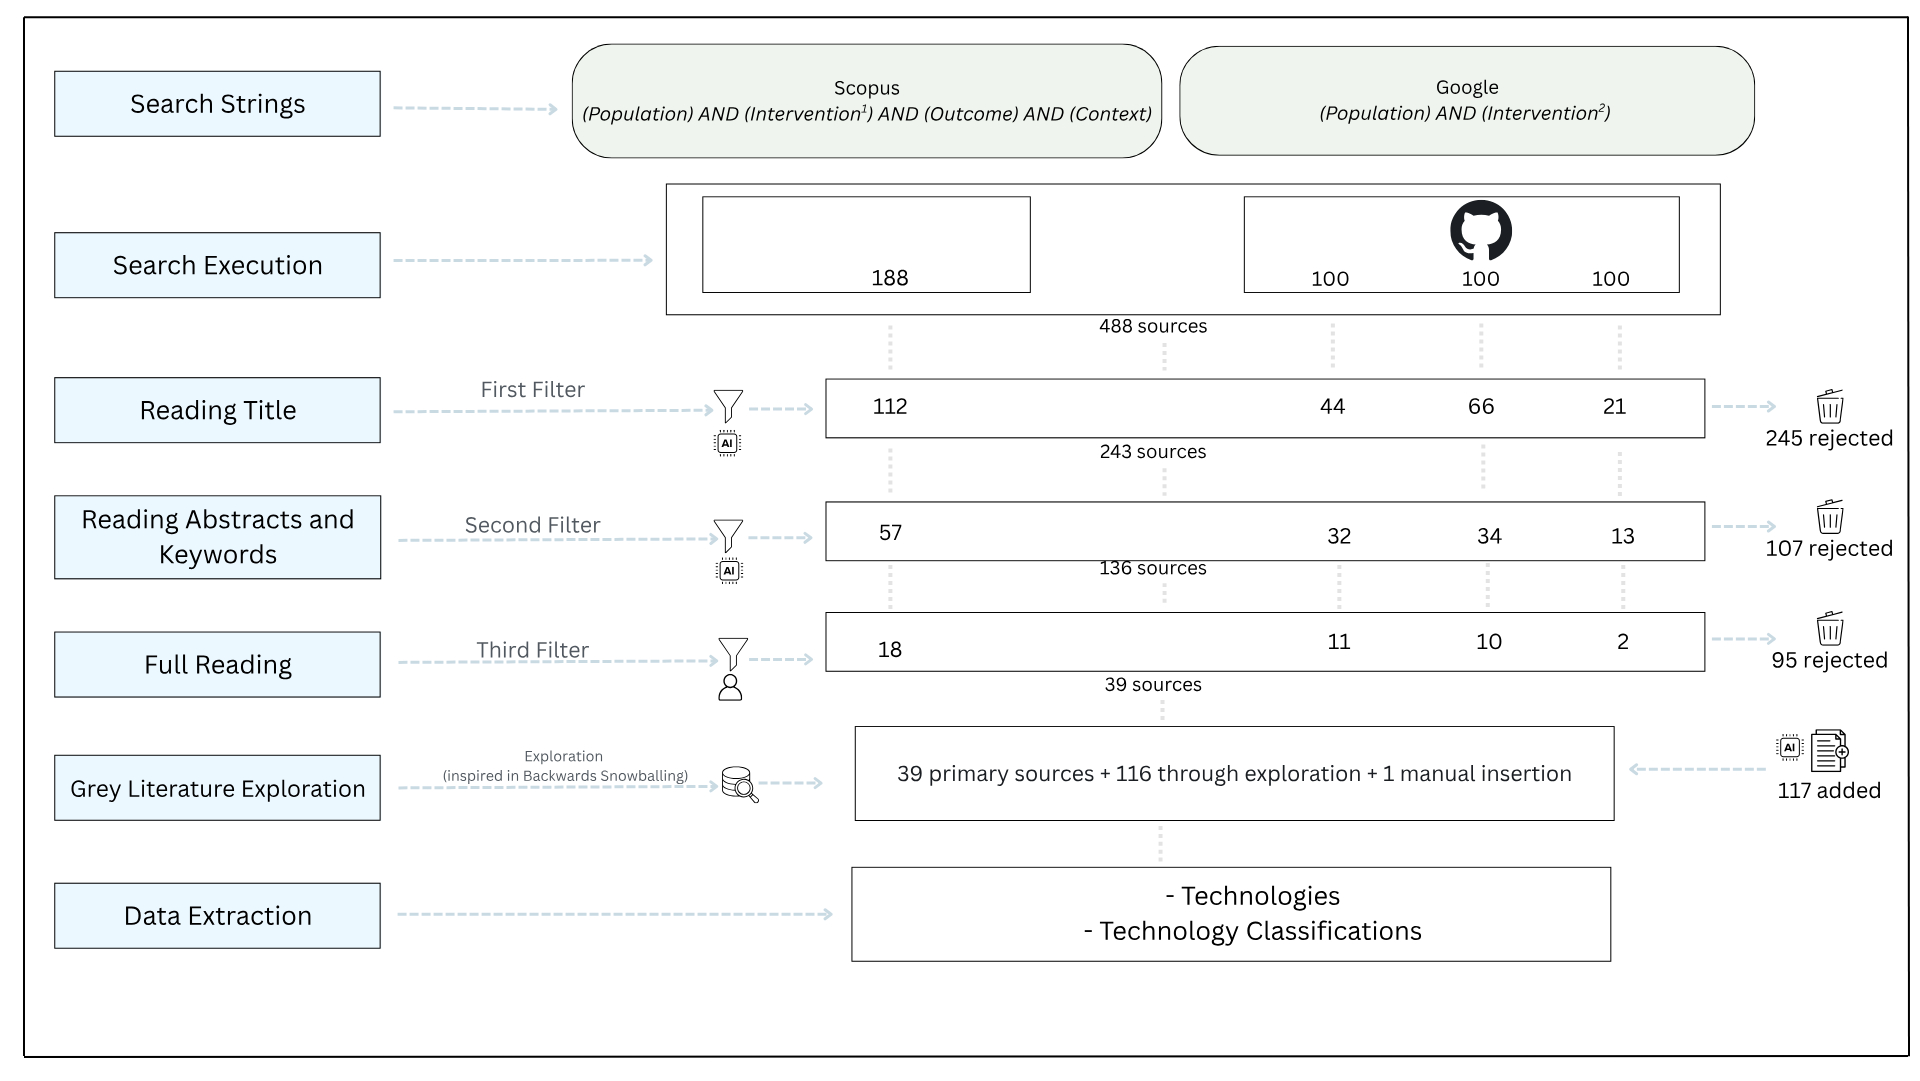
\includegraphics[width=\textwidth]{figures/search-strings.jpg}
    \caption{Methodology used in searching and filtering}
    \label{fig:workflow}
\end{center}
\end{figure*}




% =================================================================
% Results
% =================================================================
\section{Results}\label{sec:results}


A total of 488 sources were initially identified, and after applying selection criteria and expanding through exploration of grey literature, we ended up with 156 relevant results. This section presents these results organized according to the predefined research questions, referencing the identified tools by their assigned IDs, as can be seen in the Tables \ref{tab:results} and \ref{tab:results_grey} The complete analysis can be found in a Technical Report: \footnote{Technical Report: https://tinyurl.com/mtzzy2um} , which contains all sources retrieved and how they answer each RQ. 

\begin{figure}[h!]
\begin{center}
    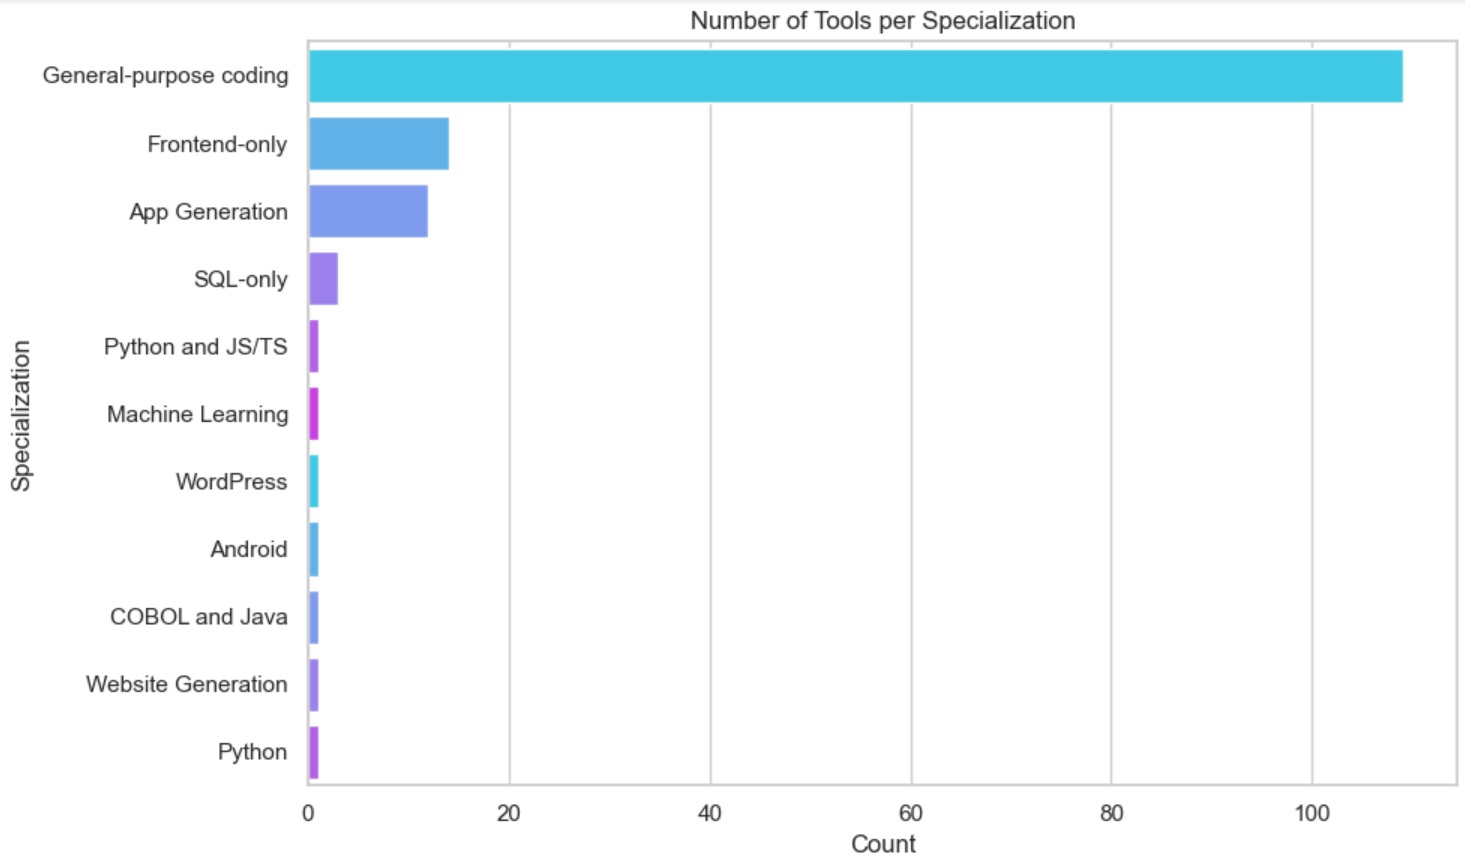
\includegraphics[width=0.48\textwidth]{figures/specialization-class.jpg}
    \caption{Distribution of tools across thematic clusters}
    \label{fig:tools_distribution}
\end{center}
\end{figure}

\subsection{RQ1a: Where can these solutions be found?}

The identified tools and technologies were primarily found across diverse channels and platforms, including official websites, dedicated repositories such as GitHub, academic databases, and specialized industry blogs. Prominent platforms for hosting these solutions include GitHub (e.g., Copilot [A01, A14, A19], StructCoder [A08]), official project websites (e.g., IBM Watsonx [A22, A35], Ansible Lightspeed [A05]), and specialized AI repositories like Hugging Face (e.g., CodeFuse-13B [A07], MarianCG [A17]). Grey literature tools such as CodeVista [A24] and Amazon Q [A25] are typically available through company websites or commercial cloud services. 

Additionally, a significant portion of grey literature is located on product and open-source portals associated with IDEs and CLIs. For instance, self-hosted assistants like Tabby [S029] on Github, editor-integrated agents such as Continue [S026] and Aider [S060], and vendor pages for JetBrains AI [S036], Gemini Code Assist [A21], and Amazon Q Developer CLI [S046]. 


\subsection{RQ1b: How can these solutions be used?}

These solutions can be categorized based on their usage contexts as follows:

\textbf{General-purpose tools:} These tools (e.g., Copilot [A01, A14, A33], Tabnine [A01], Gemini Code Assist [A21]) are integrated within Integrated Development Environments (IDEs) and are widely utilized for code generation, completion, debugging, and documentation generation across various programming languages. The general-purpose segment also includes IDE-native assistants and editor extensions such as Cursor [S001], Windsurf [S008], Zed AI [S097], Sourcegraph Cody [S014], Refact [S025], Continue [S026], and Aider [S060]. These tools offer edits, multi-file reasoning, and git-aware workflows.

\textbf{Frontend-only solutions:} Tools such as UI Pilot [S006], GitWit [S007], and Rapidpages [S084] specifically target frontend development tasks, aiding developers with tasks related to interface design and user experience improvements. This niche also encompasses design-to-code and UI generation platforms, such as v0 [S111], Uizard [S089], Kombai [S087], Magic Patterns [S085], and Galileo AI [S113], which translate wireframes or natural language prompts into React/HTML components and design artifacts.

\textbf{Application generation tools:} Replit [A28], OpenHands [S000], and GPT Web App Generator [S080] support developers in quickly creating functional prototypes or complete web and mobile applications directly from natural language descriptions. Other end-to-end generators include Bolt.new [S076], Lovable [S078], Second.dev [S104], Make Real [S081], SoftGen [S074], and Mage [S083], which scaffold multi-page apps, backends, or agents with runnable code and deployment recipes.

\textbf{Task automation solutions:} Ansible Lightspeed [A05], Grit [S065], and Shell Whiz [S054] facilitate automation of repetitive or configuration-related tasks, improving efficiency in software deployment and system management. At the CLI/infrastructure layer, Amazon Q Developer CLI [S046] and DevOpsGPT [S067] bring natural-language tasking to terminals and pipelines, while Warp [S057] and GitFluence [S055] accelerate command and Git workflow authoring.

These categories mirror the practical usage patterns reported in a recent qualitative study (\cite{klemmer2024using}), where developers highlighted use cases ranging from ideation to security mitigation practices.

\subsection{RQ1c: What is the access and usage model for these solutions and costs?}

The majority of identified tools operate under subscription or freemium models, offering limited free access to attract users. Copilot [A01, A14, A19, A23, A33] and Tabnine [A01, S030] typically follow subscription-based licensing. Platforms such as Amazon Q [A25, S041, S046] and IBM Watsonx [A22, A35] require authentication via respective cloud accounts with variable pricing based on usage. Open-source models like Code LLaMA and CodeFuse-13B [A07] are freely accessible under permissive licenses. Some simpler web-based tools like AI Code Converter [S092] offer free use, monetizing through advertisements.

Enterprise offerings increasingly provide on-premises or air-gapped deployments (e.g., Tabnine Enterprise and Ansible Lightspeed with on-prem options), while IDE add-ons like JetBrains AI Assistant follow per-seat subscriptions; Google’s Gemini Code Assist mixes a no-cost tier in Android Studio with paid tiers (Business/Enterprise) for advanced context windows and CLI features.


\subsection{RQ1d: What limitations must be considered for adopting these solutions?}

Several limitations should be considered:

\textbf{Technical limitations:} Many generative tools struggle with context awareness and producing accurate, secure code in complex scenarios (e.g., Copilot [A14, A19], CodeFuse-13B [A07]). Previous empirical studies (\cite{perry2023users, ji2024cybersecurity}) report elevated rates of vulnerabilities in AI-assisted or AI-generated code and reduced security quality among users relying on assistants.

\textbf{Operational constraints:} Most solutions, such as those from Google Cloud [A32], require stable internet connectivity and may present integration complexities within the existing infrastructure. Dependence on external APIs also imposes usage rate limits. Where data residency or connectivity constraints apply, organizations may favor self-hosted or hybrid alternatives (e.g., Tabby [S029]) and enterprise products with on-premises modes.

\textbf{Legal and ethical concerns:} Solutions handling sensitive data must comply with regulations such as GDPR. Tools that utilize external APIs or cloud-based services (IBM Watsonx [A35], Amazon Q [A25]) may pose challenges related to data privacy and intellectual property rights.

\subsection{RQ1e: What is the maturity level of these solutions?}

The identified solutions vary significantly in maturity:

\textbf{Production-ready:} Widely adopted commercial solutions such as Copilot [A01, A14, A19], Tabnine [A01], and Vertex AI [A32] demonstrate high maturity and are extensively validated in real-world settings. Other enterprise-grade assistants, such as JetBrains AI [S036], Amazon Q Developer/CLI [S041, S046], and Gemini Code Assist [A21], are also available and documented as stable, with integration across multiple IDEs.

\textbf{Experimental or beta phase:} Tools like ASPIRE [A10] and Spec2Code [A02] are in experimental stages with ongoing validation through academic and industrial case studies. Open research models for code (e.g., CodeFuse-13B [A07]) report internal deployments and evaluations.

\subsection{RQ1f: Is there technical documentation, support, or an active community?}

Most solutions provide comprehensive documentation, tutorials, and user manuals through their official channels. Copilot [A14, A19, A23, A33], IBM Watsonx [A35], and Google Cloud Vertex AI [A32] have extensive support channels, including forums, GitHub issue trackers, and customer support. 

Developer ecosystems around Continue [S026], Aider [S060], and Tabby [S029] are active and open-source-centric (docs, GitHub issues, Slack/Discord) while vendor ecosystems for JetBrains AI and Gemini Code Assist provide in-product guides, release notes, and enterprise onboarding materials.

\subsection{RQ1g: What types of target users typically engage with these solutions?}

These tools target various roles within software engineering:

\textbf{Developers and programmers:} Primary users for tools like Copilot [A01, A14], Tabnine [A01], and Gemini Code Assist [A21].

% \textbf{Testers and QA engineers:} Solutions such as ASPIRE [A10] and Calico [A06] specifically target roles involved in testing, debugging, and defect detection.

\textbf{DevOps professionals:} Task automation tools like Ansible Lightspeed [A05] and Grit [S065] benefit DevOps and infrastructure engineers directly. It must be stated that these tools do generate code and/or configuration files that automate the DevOps activities.

\subsection{RQ1h: Is there collaboration with industry through case studies or experiments?}

Some of the solutions have documented industry collaboration:

\textbf{Industrial case studies:} Tools like Spec2Code [A02] have empirical validation through industrial cases (e.g., Scania). CodeFuse-13B [A07] has been validated within AntGroup's software development processes.

\textbf{Large-scale user studies:} Ansible Lightspeed [A05] and Copilot [A14] have extensive user-based empirical studies highlighting practical industry validation and acceptance.




\begin{table*}[ht]
\centering
\caption{Technologies Employed in Software Construction: Initial Primary Sources}
\label{tab:results}
\begin{tabular}{|c|p{5cm}|p{2.5cm}||c|p{5cm}|p{2.5cm}|}
\hline
ID & Name / Technologies Identified & Specialization & ID & Name / Technologies Identified & Specialization \\
\hline
A01 & Github Copilot, Tabnine, Replit Ghostwriter, Codeium, JetBrainsAI Assistant, Kite, Visual Studio IntelliCode, Amazon CodeWhisperer, Sourcegraph Cody, Atlassian Intelligence, StarCoder, Chat-GPT & General-purpose & A21 & Gemini Code Assist & General-purpose \\
\hline
A02 & spec2code & General-purpose & A22 & IBM Watsonx & General-purpose \\
\hline
A03 & NL2Code & General-purpose & A23 & ChatGPT, Copilot & General-purpose \\
\hline
A04 & Proposed Methodology (Alpha Codium, LangChain, LangGraph, GPT), ChatGPT, Claude, ChatPDF, Perplexity & General-purpose & A24 & CodeVista & General-purpose \\
\hline
A05 & Ansible Lightspeed & Task Automation / Python & A25 & Amazon Q & General-purpose \\
\hline
A06 & Calico & General-purpose & A26 & ELEKS’ generative AI software development & General-purpose \\
\hline
A07 & CodeFuse-13B & General-purpose & A27 & ChatGPT, Copilot & General-purpose \\
\hline
A08 & StructCoder & General-purpose & A28 & Replit & App Generation \\
\hline
A09 & Codex, Copilot, PaLM2 (Pathways Language Model) & General-purpose & A29 & Shreds.AI & General-purpose \\
\hline
A10 & ASPIRE & General-purpose & A30 & ChatGPT, Copilot & General-purpose \\
\hline
A11 & Software Engineer GPT (Tailored GPT) & General-purpose & A31 & Jupyter AI & General-purpose \\
\hline
A12 & GPT-4 plus DSL & General-purpose & A32 & Google Cloud Vertex AI, Gemini models & ML \\
\hline
A13 & AskIt & General-purpose & A33 & Copilot & General-purpose \\
\hline
A14 & GitHub Copilot AI & General-purpose & A34 & Konveyor AI & General-purpose \\
\hline
A15 & The Programmer’s Assistant & General-purpose & A35 & IBM watsonx.ai & General-purpose \\
\hline
A16 & UniXcoder, CodeGPT, and InCoder & General-purpose & A36 & InCoder & General-purpose \\
\hline
A17 & MarianCG & General-purpose & A37 & Google Generative AI SDK for Kotlin & Android \\
\hline
A18 & COMPCODER & General-purpose & A38 & InCoder & General-purpose \\
\hline
A19 & Github Copliot, ChatGPT & General-purpose & A39 & CodeT5 & General-purpose \\
\hline
A20 & ChatGPT & General-purpose &  &  &  \\
\hline
\end{tabular}
\end{table*}




% --- TABELA COMPACTA ---
\begin{table*}[t]
\centering
\caption{Technologies Employed in Software Construction: Exploratory Sources (Grey Literature)}
\label{tab:results_grey}
\setlength{\tabcolsep}{3.5pt}        % compacta largura das colunas
\renewcommand{\arraystretch}{1.05}    % compacta altura das linhas
\scriptsize                           % reduz fonte apenas nesta tabela
\begin{threeparttable}
\begin{tabularx}{\textwidth}{l Y c l Y c l Y c l Y c}
\toprule
ID & Name / Technology & Sp. & ID & Name / Technology & Sp. & ID & Name / Technology & Sp. & ID & Name / Technology & Sp.\\
\midrule
\Tech{S000}{OpenHands}{\AG} & \Tech{S001}{Cursor}{\GP} & \Tech{S002}{PearAI}{\GP} & \Tech{S003}{Melty}{\GP} \\
\Tech{S004}{Replit}{\AG} & \Tech{S005}{CodeStory}{\GP} & \Tech{S006}{UI Pilot}{\FE} & \Tech{S007}{GitWit}{\FE} \\
\Tech{S008}{Windsurf}{\GP} & \Tech{S009}{Theia IDE}{\GP} & \Tech{S010}{OneCompiler}{\GP} & \Tech{S011}{trae}{\GP} \\
\Tech{S012}{Replit Ghostwriter Chat}{\GP} & \Tech{S013}{Unblocked}{\GP} & \Tech{S014}{Sourcegraph Cody}{\GP} & \Tech{S015}{Magnet}{\GP} \\
\Tech{S016}{Adrenaline}{\GP} & \Tech{S017}{Code to Flow}{\CA} & \Tech{S018}{Pieces}{\GP} & \Tech{S019}{TEXT2SQL.AI}{\SQ} \\
\Tech{S020}{SQLAI.ai}{\SQ} & \Tech{S021}{CodeWP}{\WP} & \Tech{S022}{Gru.ai}{\GP} & \Tech{S023}{GitHub Copilot}{\GP} \\
\Tech{S024}{Cline}{\GP} & \Tech{S025}{Refact AI}{\GP} & \Tech{S026}{Continue}{\GP} & \Tech{S027}{Blackbox AI}{\GP} \\
\Tech{S028}{CodeGeeX}{\GP} & \Tech{S029}{Tabby}{\GP} & \Tech{S030}{Tabnine}{\GP} & \Tech{S031}{CodeMate}{\GP} \\
\Tech{S032}{AskCodi}{\GP} & \Tech{S033}{Rubberduck}{\GP} & \Tech{S034}{CodeComplete}{\GP} & \Tech{S035}{GoCodeo}{\GP} \\
\Tech{S036}{JetBrains AI}{\GP} & \Tech{S037}{aiXcoder}{\GP} & \Tech{S038}{Sourcery}{\PJ} & \Tech{S039}{Swimm}{\GP} \\
\Tech{S040}{Supermaven}{\GP} & \Tech{S041}{Amazon Q Developer}{\GP} & \Tech{S042}{Android Studio Bot}{\AN} & \Tech{S043}{IBM watsonx Code Assistant for Z}{\CJ} \\
\Tech{S044}{EasyCode}{\GP} & \Tech{S045}{Kilo Code}{\GP} & \Tech{S046}{Amazon Q Developer CLI}{\GP} & \Tech{S047}{talk-codebase}{\GP} \\
\Tech{S048}{gptcomet}{\GP} & \Tech{S049}{poorcoder}{\GP} & \Tech{S050}{cmd-ai}{\GP} & \Tech{S051}{Memex}{\GP} \\
\Tech{S052}{Pieces}{\GP} & \Tech{S053}{Butterfish}{\GP} & \Tech{S054}{Shell Whiz}{\AU} & \Tech{S055}{GitFluence}{\AU} \\
\Tech{S056}{code-collator}{\CA} & \Tech{S057}{Warp}{\AU} & \Tech{S058}{TmuxAI}{\GP} & \Tech{S059}{Smol Developer}{\GP} \\
\Tech{S060}{Aider}{\GP} & \Tech{S061}{Blinky}{\textbf{BF}} & \Tech{S062}{Mentat}{\GP} & \Tech{S063}{GPT Engineer}{\GP} \\
\Tech{S064}{GPT Migrate}{\GP} & \Tech{S065}{Grit}{\AU} & \Tech{S066}{DemoGPT}{\AG} & \Tech{S067}{DevOpsGPT}{\AU} \\
\Tech{S068}{sudocode}{\GP} & \Tech{S069}{CodeFlash AI}{\PY} & \Tech{S070}{Micro Agent by Builder}{\GP} & \Tech{S071}{Potpie}{\GP} \\
\Tech{S071}{Claude Code}{\GP} & \Tech{S073}{Co.dev}{\GP} & \Tech{S074}{SoftGen}{\AG} & \Tech{S075}{LlamaCoder}{\GP} \\
\Tech{S076}{Bolt.new}{\AG} & \Tech{S077}{Srcbook}{\AG} & \Tech{S078}{Lovable}{\GP} & \Tech{S079}{Literally anything}{\AG} \\
\Tech{S080}{GPT Web App Generator}{\AG} & \Tech{S081}{Make Real}{\AG} & \Tech{S082}{Glowbom}{\AG} & \Tech{S083}{Mage}{\AG} \\
\Tech{S084}{Rapidpages}{\FE} & \Tech{S085}{Magic Patterns}{\FE} & \Tech{S086}{Tempo}{\FE} & \Tech{S087}{Kombai}{\FE} \\
\Tech{S088}{CodeParrot}{\FE} & \Tech{S089}{Uizard}{\FE} & \Tech{S090}{Frontly}{\FE} & \Tech{S091}{Polymet}{\FE} \\
\Tech{S092}{AI Code Convert}{\GP} & \Tech{S093}{AutoRegex}{\RE} & \Tech{S094}{ChatWithGit}{\GP} & \Tech{S095}{Code ChatGPT Plugin}{\GP} \\
\Tech{S096}{Mutable}{\GP} & \Tech{S097}{Zed}{\GP} & \Tech{S098}{CodeSquire}{\GP} & \Tech{S099}{Incognito Pilot}{\GP} \\
\Tech{S100}{Onboard}{\GP} & \Tech{S101}{Wren AI}{\SQ} & \Tech{S102}{Quack AI}{\GP} & \Tech{S103}{AskCommand}{\GP} \\
\Tech{S104}{Second.dev}{\AG} & \Tech{S105}{Factory}{\GP} & \Tech{S106}{Pico}{\AG} & \Tech{S107}{e2b Fragments}{\GP} \\
\Tech{S108}{Bolt.diy}{\GP} & \Tech{S109}{Marblism}{\AG} & \Tech{S110}{ScrollHub}{\WG} & \Tech{S111}{v0}{\FE} \\
\Tech{S112}{Rendition Create}{\FE} & \Tech{S113}{Galileo AI}{\FE} & \Tech{S114}{BoringUi}{\FE} & \Tech{S115}{CodePal}{\GP} \\
\Tech{S116}{AI Code Playground}{\GP} & & & & & & & & & & & \\
\bottomrule
\end{tabularx}

\vspace{2pt}
\footnotesize
\textbf{Legend.} \GP{}=General-purpose; \AG{}=App Generation; \FE{}=Frontend-only; \AU{}=Automation; \CA{}=Code Analysis; \SQ{}=SQL-only; \WP{}=WordPress; \PY{}=Python; \AN{}=Android; \CJ{}=COBOL \& Java; \RE{}=Regex; \WG{}=Website Generation; \textbf{BF}=Backend-focused; \PJ{}=Python \& JS/TS.
\end{threeparttable}
\end{table*}





% \begin{table*}[ht]\label{table_s}
% \centering
% \caption{Technologies Employed in Software Construction: Exploratory Sources (Grey Literature)}
% \begin{tabular}{|c|p{5cm}|p{2.5cm}||c|p{5cm}|p{2.5cm}|}
% \hline
% ID & Name / Technologies Identified & Specialization & ID & Name / Technologies Identified & Specialization \\
% \hline
% S000 & OpenHands & App Generation & S059 & Smol Developer & General-purpose \\
% \hline
% S001 & Cursor & General-purpose & S060 & Aider & General-purpose \\
% \hline
% S002 & PearAI & General-purpose & S061 & Blinky & Backend focused \\
% \hline
% S003 & Melty & General-purpose & S062 & Mentat & General-purpose \\
% \hline
% S004 & Replit & App Generation & S063 & GPT Engineer & General-purpose \\
% \hline
% S005 & CodeStory & General-purpose & S064 & GPT Migrate & General-purpose \\
% \hline
% S006 & UI Pilot & Frontend-only & S065 & Grit & Automation \\
% \hline
% S007 & GitWit & Frontend-only & S066 & DemoGPT & App Generation \\
% \hline
% S008 & Windsurf & General-purpose & S067 & DevOpsGPT & Automation \\
% \hline
% S009 & Theia IDE & General-purpose & S068 & sudocode & General-purpose \\
% \hline
% S010 & OneCompiler & General-purpose & S069 & CodeFlash AI & Python \\
% \hline
% S011 & trae & General-purpose & S070 & Micro Agent by Builder & General-purpose \\
% \hline
% S012 & Replit Ghostwriter Chat & General-purpose & S071 & Potpie & General-purpose \\
% \hline
% S013 & Unblocked & General-purpose & S071 & Claude Code & General-purpose \\
% \hline
% S014 & Sourcegraph Cody & General-purpose & S073 & Co.dev & General-purpose \\
% \hline
% S015 & Magnet & General-purpose & S074 & SoftGen & App Generation \\
% \hline
% S016 & Adrenaline & General-purpose & S075 & LlamaCoder & General-purpose \\
% \hline
% S017 & Code to Flow & Code Analysis & S076 & Bolt.new & App Generation \\
% \hline
% S018 & Pieces & General-purpose & S077 & Srcbook & App Generation \\
% \hline
% S019 & TEXT2SQL.AI & SQL-only & S078 & Lovable & General-purpose \\
% \hline
% S020 & SQLAI.ai & SQL-only & S079 & Literally anything & App Generation \\
% \hline
% S021 & CodeWP & WordPress & S080 & GPT Web App Generator & App Generation \\
% \hline
% S022 & Gru.ai & General-purpose & S081 & Make Real & App Generation \\
% \hline
% S023 & GitHub Copilot & General-purpose & S082 & Glowbom & App Generation \\
% \hline
% S024 & Cline & General-purpose & S083 & Mage & App Generation \\
% \hline
% S025 & Refact AI & General-purpose & S084 & Rapidpages & Frontend-only \\
% \hline
% S026 & Continue & General-purpose & S085 & Magic Patterns & Frontend-only \\
% \hline
% S027 & Blackbox AI & General-purpose & S086 & Tempo & Frontend-only \\
% \hline
% S028 & CodeGeeX & General-purpose & S087 & Kombai & Frontend-only \\
% \hline
% S029 & Tabby & General-purpose & S088 & CodeParrot & Frontend-only \\
% \hline
% S030 & Tabnine & General-purpose & S089 & Uizard & Frontend-only \\
% \hline
% S031 & CodeMate & General-purpose & S090 & Frontly & Frontend-only \\
% \hline
% S032 & AskCodi & General-purpose & S091 & Polymet & Frontend-only \\
% \hline
% S033 & Rubberduck & General-purpose & S092 & AI Code Convert & General-purpose \\
% \hline
% S034 & CodeComplete & General-purpose & S093 & AutoRegex & Regex \\
% \hline
% S035 & GoCodeo & General-purpose & S094 & ChatWithGit & General-purpose \\
% \hline
% S036 & JetBrains AI & General-purpose & S095 & Code ChatGPT Plugin & General-purpose \\
% \hline
% S037 & aiXcoder & General-purpose & S096 & Mutable & General-purpose \\
% \hline
% S038 & Sourcery & Python and JS/TS & S097 & Zed & General-purpose \\
% \hline
% S039 & Swimm & General-purpose & S098 & CodeSquire & General-purpose \\
% \hline
% S040 & Supermaven & General-purpose & S099 & Incognito Pilot & General-purpose \\
% \hline
% S041 & Amazon Q Developer & General-purpose & S100 & Onboard & General-purpose \\
% \hline
% S042 & Android Studio Bot & Android & S101 & Wren AI & SQL-only \\
% \hline
% S043 & IBM watsonx Code Assistant for Z & COBOL and Java & S102 & Quack AI & General-purpose \\
% \hline
% S044 & EasyCode & General-purpose & S103 & AskCommand & General-purpose \\
% \hline
% S045 & Kilo Code & General-purpose & S104 & Second.dev & App Generation \\
% \hline
% S046 & Amazon Q Developer CLI & General-purpose & S105 & Factory & General-purpose \\
% \hline
% S047 & talk-codebase & General-purpose & S106 & Pico & App Generation \\
% \hline
% S048 & gptcomet & General-purpose & S107 & e2b Fragments & General-purpose \\
% \hline
% S049 & poorcoder & General-purpose & S108 & Bolt.diy & General-purpose \\
% \hline
% S050 & cmd-ai & General-purpose & S109 & Marblism & App Generation \\
% \hline
% S051 & Memex & General-purpose & S110 & ScrollHub & Website Generation \\
% \hline
% S052 & Pieces & General-purpose & S111 & v0 & Frontend-only \\
% \hline
% S053 & Butterfish & General-purpose & S112 & Rendition Create & Frontend-only \\
% \hline
% S054 & Shell Whiz & Automation & S113 & Galileo AI & Frontend-only \\
% \hline
% S055 & GitFluence & Automation & S114 & BoringUi & Frontend-only \\
% \hline
% S056 & code-collator & Code Analysis & S115 & CodePal & General-purpose \\
% \hline
% S057 & Warp & Automation & S116 & AI Code Playground & General-purpose \\
% \hline
% S058 & TmuxAI & General-purpose &  &  &  \\
% \hline
% \end{tabular}
% \end{table*}





% =================================================================
% Discussion
% =================================================================
% \section{Discussion}\label{sec:discussion}
% \subsection{Maturity and Adoption}

Beyond the coarse divide between prototypes and commercial products, maturity appears uneven across workflow stages. Assistants embedded in IDEs and CI environments tend to exhibit stronger reliability guarantees, clearer telemetry, and better policy controls, while end-to-end “app generators” and agentic toolchains still face churn in model backends and dependency stability. Reported productivity gains are promising but heterogeneous: controlled and field studies find time savings and reduced cognitive load, yet effects depend on task complexity, developer expertise, and the need for architectural reasoning \cite{peng2023impact,becker2025measuring}. Adoption is strongly mediated by organizational governance. Interviews indicate enthusiasm tempered by concerns about data exposure, provenance, and compliance, which shape procurement choices such as on-premises deployment, audit logging, and approved prompt patterns \cite{klemmer2024using}. Security findings further motivate cautious rollout and targeted training, given evidence that AI-assisted code can introduce or preserve vulnerabilities if safeguards and review practices are weak \cite{perry2023users,asare2024user}. In sum, the most mature deployments couple tool capability with operational guardrails and continuous evaluation aligned with software engineering guidance syntheses \cite{hou2024large}.

\subsection{Target Roles and Usage Models}

A broader role spectrum is emerging as capabilities move upstream and downstream of coding. Early evidence from requirements engineering suggests that LLMs can aid in drafting, refinement, and traceability when paired with structured prompts and review checkpoints, thereby inviting participation from analysts and domain experts under human-in-the-loop regimes (Cheng, 2024; generative). On the operations side, code-generating services for automation illustrate how DevOps teams adopt assistants through reproducible templates and policy-constrained suggestions that fit existing pipelines \cite{sahoo2024ansible}. Across roles, two usage models recur: co-creation, where practitioners iterate within familiar tools with immediate feedback and citations, and delegation, where agents orchestrate multi-step tasks under explicit constraints and post-hoc verification. Organizations that differentiate these modes, provide security-aware guidance, and instrument review workflows report smoother onboarding and more consistent outcomes \cite{klemmer2024using}.

% \subsection{Challenges and Limitations}
% Significant limitations include context-window restrictions, hallucinations, incomplete dependency resolution, and the requirement of post-editing by users.


% Ethical and legal concerns persist around code provenance, data privacy, and intellectual property.



% =================================================================
% Future Work
% =================================================================
\section{Future Work and Threats to Validity}\label{sec:futurework}
\subsection{Future Work}

Future work may expand along several complementary directions. First, the review's scope can be broadened by incorporating additional data sources, such as querying repositories like arXiv or GitHub using their native APIs with various filters, to identify a wider array of Generative AI tools applicable to software engineering. Employing techniques similar to those used in the AgentOps study \cite{dong2024taxonomy}, particularly leveraging repository metrics (e.g., stars, forks), can enhance content relevancy by filtering out redundant or derivative repositories. Each API has its own particularities, such as the GitHub API, which allows fewer characters and logic connectors, requiring a different search string.

Introducing automatic feedback by integrating user-driven annotations or behavioral traces (e.g., GitHub issue discussions, Stack Overflow activities) could iteratively refine the relevance, accuracy, and usability of the cataloged tools. This continuous feedback approach ensures an evolving and highly practical resource for both academia and industry.

Finally, the filtering pipeline can be augmented with reinforcement learning or optimized using prompting techniques. These advanced mechanisms could continuously improve classification accuracy and adaptability by leveraging incremental validation results from replication studies.


\subsection{Threats to Validity}

To assess the threats to validity in this study, we applied threat categories tailored for secondary studies in computing as recommended by \cite{ampatzoglou2019identifying}. Specifically, we recognized threats relating to (i) scope definition when crafting search strings, (ii) accuracy and objectivity during data extraction and description of observations, and (iii) researcher bias.

To mitigate threats arising from the limited research scope, we constructed our search strings using the method described in \cite{garousi2020grey}, which were iteratively refined through pilot searches before final adoption. To address concerns regarding accuracy and objectivity, we employed and validated a structured data extraction protocol to facilitate systematic recording and the transparent verification of results.

Researcher bias poses a particular challenge when selecting and interpreting grey literature, due to its often ambiguous or incomplete nature. To address this, we included additional relevant sources identified through links within the grey literature itself, thus broadening the initial coverage. However, it should be noted that our specific selection of GPT-4.1 inherently introduces a bias, as language models were not comprehensively evaluated, which may limit the generalizability of our findings.

Finally, the generalizability of our conclusions may be affected by the rapidly evolving landscape of Generative AI technologies. Thus, continuous monitoring, updates, and periodic re-evaluations are essential to preserve the relevance and applicability of our results. For instance, in our review, we found some tools that were no longer maintained and some deprecated repositories that were initially made public just a few years ago, illustrating the rapid pace of change in this domain. 




% =================================================================
% Final Remarks
% =================================================================
\section{Final Remarks}\label{sec:finalremarks}
This Rapid Multivocal Review highlights a rapidly expanding landscape of Generative AI tools applicable to software construction, as detailed throughout Section \ref{sec:results} where we systematically categorize and analyze these tools. Section \ref{sec:futurework} critically addresses inherent validity threats, including scope definition, objectivity in data extraction, and researcher bias. Despite significant advancements, overall, we emphasize ongoing challenges in integrating these tools into reliable software development workflows, as some of these tools are still very bare bones and often require extensive environment configuration, which is probably why ChatGPT ends up being the tool that appears the most, due to being easier for the end user. Section \ref{sec:futurework} also outlines future research directions, advocating for the extension of repository searches, the employment of advanced filtering techniques, and the continuous validation of the applicability and maturity of tools. Ultimately, this work provides a structured, evidence-based foundation that encourages deeper academic-industry collaborations to exploit the transformative potential of Generative AI fully.

% \begin{table}[h!]
%     \centering
%     \caption{Examples of Tools by Software Engineering Activity}
%     \begin{tabular}{|l|l|}
%         \hline
%         \textbf{Activity} & \textbf{Example Tools} \\
%         \hline
%         Code Generation & Copilot, Codeium, Ghostwriter \\
%         Test Creation & TestPilot, GPT-TestGen \\
%         Refactoring & StarCoder, CodeT5+ \\
%         Requirement Parsing & Software Engineer GPT, NL2Code \\
%         Bug Fixing & Calico, ASPIRE \\
%         \hline
%     \end{tabular}
%     \label{tab:tools_by_activity}
% \end{table}

% =================================================================
% Acknowledgements
% =================================================================
\section{Acknowledgements}\label{sec:acknowledgements}
\begin{declarations}

\begin{funding}
This study was financed in part by the Conselho Nacional de Desenvolvimento Científico e Tecnológico – Brasil (CNPq, Grant 305701/2022-3) and the Fundação Carlos Chagas Filho de Amparo à Pesquisa do Estado do Rio de Janeiro – FAPERJ (Grant E-26/204.310/2024) for partial support.
\end{funding}


\begin{interests}
The authors declare that they have no competing interests.
\end{interests}

\begin{materials}
The data and other materials created and/or used in this literature review
are available at DOI: 10.5281/zenodo.17465501.
\end{materials}

\begin{aitools}
We acknowledge using ChatGPT tools to support the creative process,
translation, and rewriting to improve text clarity as well as a part of the conducted experiment. We reviewed all outputs to ensure alignment with our original intent.
\end{aitools}

\end{declarations}

% =================================================================
% Bibliography
% =================================================================
\bibliographystyle{apalike-sol}
\bibliography{9-refs}

\end{document}
